\documentclass[letterpaper]{article} %
\usepackage{aaai23}  %
\usepackage{times}  %
\usepackage{helvet}  %
\usepackage{courier}  %
\usepackage[hyphens]{url}  %
\usepackage{graphicx} %
\urlstyle{rm} %
\def\UrlFont{\rm}  %
\usepackage{natbib}  %
\usepackage{caption} %
\frenchspacing  %
\setlength{\pdfpagewidth}{8.5in}  %
\setlength{\pdfpageheight}{11in}  %
\usepackage{algorithm}
\usepackage{algorithmic}

\usepackage{newfloat}
\usepackage{listings}
\DeclareCaptionStyle{ruled}{labelfont=normalfont,labelsep=colon,strut=off} %
\lstset{%
	basicstyle={\footnotesize\ttfamily},%
	numbers=left,numberstyle=\footnotesize,xleftmargin=2em,%
	aboveskip=0pt,belowskip=0pt,%
	showstringspaces=false,tabsize=2,breaklines=true}
\floatstyle{ruled}
\newfloat{listing}{tb}{lst}{}
\floatname{listing}{Listing}


\setcounter{secnumdepth}{2} %


%%%%% NEW MATH DEFINITIONS %%%%%

\usepackage{amsmath,amsfonts,bm}

\def\Eqref#1{Eq.~\eqref{#1}}
\def\Tabref#1{Table~\ref{#1}}
\def\eps{{\epsilon}}


% Random variables
\def\reta{{\textnormal{$\eta$}}}
\def\ra{{\textnormal{a}}}
\def\rT{{\textnormal{T}}}
\def\rL{{\textnormal{L}}}
\def\rb{{\textnormal{b}}}
\def\rc{{\textnormal{c}}}
\def\rd{{\textnormal{d}}}
\def\re{{\textnormal{e}}}
\def\rf{{\textnormal{f}}}
\def\rg{{\textnormal{g}}}
\def\rh{{\textnormal{h}}}
\def\ri{{\textnormal{i}}}
\def\rj{{\textnormal{j}}}
\def\rk{{\textnormal{k}}}
\def\rl{{\textnormal{l}}}
% rm is already a command, just don't name any random variables m
\def\rn{{\textnormal{n}}}
\def\ro{{\textnormal{o}}}
\def\rp{{\textnormal{p}}}
\def\rq{{\textnormal{q}}}
\def\rr{{\textnormal{r}}}
\def\rs{{\textnormal{s}}}
\def\rt{{\textnormal{t}}}
\def\ru{{\textnormal{u}}}
\def\rv{{\textnormal{v}}}
\def\rw{{\textnormal{w}}}
\def\rx{{\textnormal{x}}}
\def\ry{{\textnormal{y}}}
\def\rz{{\textnormal{z}}}

% Random vectors
\def\rvepsilon{{\mathbf{\epsilon}}}
\def\rvtheta{{\mathbf{\theta}}}
\def\rva{{\mathbf{a}}}
\def\rvb{{\mathbf{b}}}
\def\rvc{{\mathbf{c}}}
\def\rvd{{\mathbf{d}}}
\def\rve{{\mathbf{e}}}
\def\rvf{{\mathbf{f}}}
\def\rvg{{\mathbf{g}}}
\def\rvh{{\mathbf{h}}}
\def\rvu{{\mathbf{i}}}
\def\rvj{{\mathbf{j}}}
\def\rvk{{\mathbf{k}}}
\def\rvl{{\mathbf{l}}}
\def\rvm{{\mathbf{m}}}
\def\rvn{{\mathbf{n}}}
\def\rvo{{\mathbf{o}}}
\def\rvp{{\mathbf{p}}}
\def\rvq{{\mathbf{q}}}
\def\rvr{{\mathbf{r}}}
\def\rvs{{\mathbf{s}}}
\def\rvt{{\mathbf{t}}}
\def\rvu{{\mathbf{u}}}
\def\rvv{{\mathbf{v}}}
\def\rvw{{\mathbf{w}}}
\def\rvx{{\mathbf{x}}}
\def\rvy{{\mathbf{y}}}
\def\rvz{{\mathbf{z}}}

% Elements of random vectors
\def\erva{{\textnormal{a}}}
\def\ervb{{\textnormal{b}}}
\def\ervc{{\textnormal{c}}}
\def\ervd{{\textnormal{d}}}
\def\erve{{\textnormal{e}}}
\def\ervf{{\textnormal{f}}}
\def\ervg{{\textnormal{g}}}
\def\ervh{{\textnormal{h}}}
\def\ervi{{\textnormal{i}}}
\def\ervj{{\textnormal{j}}}
\def\ervk{{\textnormal{k}}}
\def\ervl{{\textnormal{l}}}
\def\ervm{{\textnormal{m}}}
\def\ervn{{\textnormal{n}}}
\def\ervo{{\textnormal{o}}}
\def\ervp{{\textnormal{p}}}
\def\ervq{{\textnormal{q}}}
\def\ervr{{\textnormal{r}}}
\def\ervs{{\textnormal{s}}}
\def\ervt{{\textnormal{t}}}
\def\ervu{{\textnormal{u}}}
\def\ervv{{\textnormal{v}}}
\def\ervw{{\textnormal{w}}}
\def\ervx{{\textnormal{x}}}
\def\ervy{{\textnormal{y}}}
\def\ervz{{\textnormal{z}}}

% Random matrices
\def\rmA{{\mathbf{A}}}
\def\rmB{{\mathbf{B}}}
\def\rmC{{\mathbf{C}}}
\def\rmD{{\mathbf{D}}}
\def\rmE{{\mathbf{E}}}
\def\rmF{{\mathbf{F}}}
\def\rmG{{\mathbf{G}}}
\def\rmH{{\mathbf{H}}}
\def\rmI{{\mathbf{I}}}
\def\rmJ{{\mathbf{J}}}
\def\rmK{{\mathbf{K}}}
\def\rmL{{\mathbf{L}}}
\def\rmM{{\mathbf{M}}}
\def\rmN{{\mathbf{N}}}
\def\rmO{{\mathbf{O}}}
\def\rmP{{\mathbf{P}}}
\def\rmQ{{\mathbf{Q}}}
\def\rmR{{\mathbf{R}}}
\def\rmS{{\mathbf{S}}}
\def\rmT{{\mathbf{T}}}
\def\rmU{{\mathbf{U}}}
\def\rmV{{\mathbf{V}}}
\def\rmW{{\mathbf{W}}}
\def\rmX{{\mathbf{X}}}
\def\rmY{{\mathbf{Y}}}
\def\rmZ{{\mathbf{Z}}}

% Elements of random matrices
\def\ermA{{\textnormal{A}}}
\def\ermB{{\textnormal{B}}}
\def\ermC{{\textnormal{C}}}
\def\ermD{{\textnormal{D}}}
\def\ermE{{\textnormal{E}}}
\def\ermF{{\textnormal{F}}}
\def\ermG{{\textnormal{G}}}
\def\ermH{{\textnormal{H}}}
\def\ermI{{\textnormal{I}}}
\def\ermJ{{\textnormal{J}}}
\def\ermK{{\textnormal{K}}}
\def\ermL{{\textnormal{L}}}
\def\ermM{{\textnormal{M}}}
\def\ermN{{\textnormal{N}}}
\def\ermO{{\textnormal{O}}}
\def\ermP{{\textnormal{P}}}
\def\ermQ{{\textnormal{Q}}}
\def\ermR{{\textnormal{R}}}
\def\ermS{{\textnormal{S}}}
\def\ermT{{\textnormal{T}}}
\def\ermU{{\textnormal{U}}}
\def\ermV{{\textnormal{V}}}
\def\ermW{{\textnormal{W}}}
\def\ermX{{\textnormal{X}}}
\def\ermY{{\textnormal{Y}}}
\def\ermZ{{\textnormal{Z}}}

% Vectors
\def\vzero{{\bm{0}}}
\def\vone{{\bm{1}}}
\def\vmu{{\bm{\mu}}}
\def\vtheta{{\bm{\theta}}}
\def\va{{\bm{a}}}
\def\vB{{\bm{B}}}
\def\vb{{\bm{b}}}
\def\vc{{\bm{c}}}
\def\vd{{\bm{d}}}
\def\ve{{\bm{e}}}
\def\vf{{\bm{f}}}
\def\vg{{\bm{g}}}
\def\vh{{\bm{h}}}
\def\vi{{\bm{i}}}
\def\vj{{\bm{j}}}
\def\vk{{\bm{k}}}
\def\vl{{\bm{l}}}
\def\vm{{\bm{m}}}
\def\vn{{\bm{n}}}
\def\vo{{\bm{o}}}
\def\vp{{\bm{p}}}
\def\vq{{\bm{q}}}
\def\vr{{\bm{r}}}
\def\vs{{\bm{s}}}
\def\vt{{\bm{t}}}
\def\vu{{\bm{u}}}
\def\vv{{\bm{v}}}
\def\vw{{\bm{w}}}
\def\vx{{\bm{x}}}
\def\vy{{\bm{y}}}
\def\vz{{\bm{z}}}


% Elements of vectors
\def\evalpha{{\alpha}}
\def\evbeta{{\beta}}
\def\evepsilon{{\epsilon}}
\def\evlambda{{\lambda}}
\def\evomega{{\omega}}
\def\evmu{{\mu}}
\def\evpsi{{\psi}}
\def\evsigma{{\sigma}}
\def\evtheta{{\theta}}
\def\eva{{a}}
\def\evb{{b}}
\def\evc{{c}}
\def\evd{{d}}
\def\eve{{e}}
\def\evf{{f}}
\def\evg{{g}}
\def\evh{{h}}
\def\evi{{i}}
\def\evj{{j}}
\def\evk{{k}}
\def\evl{{l}}
\def\evm{{m}}
\def\evn{{n}}
\def\evo{{o}}
\def\evp{{p}}
\def\evq{{q}}
\def\evr{{r}}
\def\evs{{s}}
\def\evt{{t}}
\def\evu{{u}}
\def\evv{{v}}
\def\evw{{w}}
\def\evx{{x}}
\def\evy{{y}}
\def\evz{{z}}

% Matrix
\def\mA{{\bm{A}}}
\def\mB{{\bm{B}}}
\def\mC{{\bm{C}}}
\def\mD{{\bm{D}}}
\def\mE{{\bm{E}}}
\def\mF{{\bm{F}}}
\def\mG{{\bm{G}}}
\def\mH{{\bm{H}}}
\def\mI{{\bm{I}}}
\def\mJ{{\bm{J}}}
\def\mK{{\bm{K}}}
\def\mL{{\bm{L}}}
\def\mM{{\bm{M}}}
\def\mN{{\bm{N}}}
\def\mO{{\bm{O}}}
\def\mP{{\bm{P}}}
\def\mQ{{\bm{Q}}}
\def\mR{{\bm{R}}}
\def\mS{{\bm{S}}}
\def\mT{{\bm{T}}}
\def\mU{{\bm{U}}}
\def\mV{{\bm{V}}}
\def\mW{{\bm{W}}}
\def\mX{{\bm{X}}}
\def\mY{{\bm{Y}}}
\def\mZ{{\bm{Z}}}
\def\mBeta{{\bm{\beta}}}
\def\mPhi{{\bm{\Phi}}}
\def\mLambda{{\bm{\Lambda}}}
\def\mSigma{{\bm{\Sigma}}}

% Tensor
\DeclareMathAlphabet{\mathsfit}{\encodingdefault}{\sfdefault}{m}{sl}
\SetMathAlphabet{\mathsfit}{bold}{\encodingdefault}{\sfdefault}{bx}{n}
\newcommand{\tens}[1]{\bm{\mathsfit{#1}}}
\def\tA{{\tens{A}}}
\def\tB{{\tens{B}}}
\def\tC{{\tens{C}}}
\def\tD{{\tens{D}}}
\def\tE{{\tens{E}}}
\def\tF{{\tens{F}}}
\def\tG{{\tens{G}}}
\def\tH{{\tens{H}}}
\def\tI{{\tens{I}}}
\def\tJ{{\tens{J}}}
\def\tK{{\tens{K}}}
\def\tL{{\tens{L}}}
\def\tM{{\tens{M}}}
\def\tN{{\tens{N}}}
\def\tO{{\tens{O}}}
\def\tP{{\tens{P}}}
\def\tQ{{\tens{Q}}}
\def\tR{{\tens{R}}}
\def\tS{{\tens{S}}}
\def\tT{{\tens{T}}}
\def\tU{{\tens{U}}}
\def\tV{{\tens{V}}}
\def\tW{{\tens{W}}}
\def\tX{{\tens{X}}}
\def\tY{{\tens{Y}}}
\def\tZ{{\tens{Z}}}


% Graph
\def\gA{{\mathcal{A}}}
\def\gB{{\mathcal{B}}}
\def\gC{{\mathcal{C}}}
\def\gD{{\mathcal{D}}}
\def\gE{{\mathcal{E}}}
\def\gF{{\mathcal{F}}}
\def\gG{{\mathcal{G}}}
\def\gH{{\mathcal{H}}}
\def\gI{{\mathcal{I}}}
\def\gJ{{\mathcal{J}}}
\def\gK{{\mathcal{K}}}
\def\gL{{\mathcal{L}}}
\def\gM{{\mathcal{M}}}
\def\gN{{\mathcal{N}}}
\def\gO{{\mathcal{O}}}
\def\gP{{\mathcal{P}}}
\def\gQ{{\mathcal{Q}}}
\def\gR{{\mathcal{R}}}
\def\gS{{\mathcal{S}}}
\def\gT{{\mathcal{T}}}
\def\gU{{\mathcal{U}}}
\def\gV{{\mathcal{V}}}
\def\gW{{\mathcal{W}}}
\def\gX{{\mathcal{X}}}
\def\gY{{\mathcal{Y}}}
\def\gZ{{\mathcal{Z}}}

% Sets
\def\sA{{\mathbb{A}}}
\def\sB{{\mathbb{B}}}
\def\sC{{\mathbb{C}}}
\def\sD{{\mathbb{D}}}
\def\sE{{\mathbb{E}}}
% Don't use a set called E, because this would be the same as our symbol
% for expectation.
\def\sF{{\mathbb{F}}}
\def\sG{{\mathbb{G}}}
\def\sH{{\mathbb{H}}}
\def\sI{{\mathbb{I}}}
\def\sJ{{\mathbb{J}}}
\def\sK{{\mathbb{K}}}
\def\sL{{\mathbb{L}}}
\def\sM{{\mathbb{M}}}
\def\sN{{\mathbb{N}}}
\def\sO{{\mathbb{O}}}
\def\sP{{\mathbb{P}}}
\def\sQ{{\mathbb{Q}}}
\def\sR{{\mathbb{R}}}
\def\sS{{\mathbb{S}}}
\def\sT{{\mathbb{T}}}
\def\sU{{\mathbb{U}}}
\def\sV{{\mathbb{V}}}
\def\sW{{\mathbb{W}}}
\def\sX{{\mathbb{X}}}
\def\sY{{\mathbb{Y}}}
\def\sZ{{\mathbb{Z}}}

% Entries of a matrix
\def\emLambda{{\Lambda}}
\def\emA{{A}}
\def\emB{{B}}
\def\emC{{C}}
\def\emD{{D}}
\def\emE{{E}}
\def\emF{{F}}
\def\emG{{G}}
\def\emH{{H}}
\def\emI{{I}}
\def\emJ{{J}}
\def\emK{{K}}
\def\emL{{L}}
\def\emM{{M}}
\def\emN{{N}}
\def\emO{{O}}
\def\emP{{P}}
\def\emQ{{Q}}
\def\emR{{R}}
\def\emS{{S}}
\def\emT{{T}}
\def\emU{{U}}
\def\emV{{V}}
\def\emW{{W}}
\def\emX{{X}}
\def\emY{{Y}}
\def\emZ{{Z}}
\def\emSigma{{\Sigma}}

% entries of a tensor
% Same font as tensor, without \bm wrapper
\newcommand{\etens}[1]{\mathsfit{#1}}
\def\etLambda{{\etens{\Lambda}}}
\def\etA{{\etens{A}}}
\def\etB{{\etens{B}}}
\def\etC{{\etens{C}}}
\def\etD{{\etens{D}}}
\def\etE{{\etens{E}}}
\def\etF{{\etens{F}}}
\def\etG{{\etens{G}}}
\def\etH{{\etens{H}}}
\def\etI{{\etens{I}}}
\def\etJ{{\etens{J}}}
\def\etK{{\etens{K}}}
\def\etL{{\etens{L}}}
\def\etM{{\etens{M}}}
\def\etN{{\etens{N}}}
\def\etO{{\etens{O}}}
\def\etP{{\etens{P}}}
\def\etQ{{\etens{Q}}}
\def\etR{{\etens{R}}}
\def\etS{{\etens{S}}}
\def\etT{{\etens{T}}}
\def\etU{{\etens{U}}}
\def\etV{{\etens{V}}}
\def\etW{{\etens{W}}}
\def\etX{{\etens{X}}}
\def\etY{{\etens{Y}}}
\def\etZ{{\etens{Z}}}

% The true underlying data generating distribution
\newcommand{\pdata}{p_{\rm{data}}}
% The empirical distribution defined by the training set
\newcommand{\ptrain}{\hat{p}_{\rm{data}}}
\newcommand{\Ptrain}{\hat{P}_{\rm{data}}}
% The model distribution
\newcommand{\pmodel}{p_{\rm{model}}}
\newcommand{\Pmodel}{P_{\rm{model}}}
\newcommand{\ptildemodel}{\tilde{p}_{\rm{model}}}
% Stochastic autoencoder distributions
\newcommand{\pencode}{p_{\rm{encoder}}}
\newcommand{\pdecode}{p_{\rm{decoder}}}
\newcommand{\precons}{p_{\rm{reconstruct}}}
\newcommand{\laplace}{\mathrm{Laplace}} % Laplace distribution
\newcommand{\E}{\mathbb{E}}
\newcommand{\Ls}{\mathcal{L}}
\newcommand{\R}{\mathbb{R}}
\newcommand{\emp}{\tilde{p}}
\newcommand{\lr}{\alpha}
\newcommand{\reg}{\lambda}
\newcommand{\rect}{\mathrm{rectifier}}
\newcommand{\softmax}{\mathrm{softmax}}
\newcommand{\sigmoid}{\sigma}
\newcommand{\softplus}{\zeta}
\newcommand{\KL}{D_{\mathrm{KL}}}
\newcommand{\Var}{\mathrm{Var}}
\newcommand{\standarderror}{\mathrm{SE}}
\newcommand{\Cov}{\mathrm{Cov}}
% Wolfram Mathworld says $L^2$ is for function spaces and $\ell^2$ is for vectors
% But then they seem to use $L^2$ for vectors throughout the site, and so does
% wikipedia.
\newcommand{\normlzero}{L^0}
\newcommand{\normlone}{L^1}
\newcommand{\normltwo}{L^2}
\newcommand{\normlp}{L^p}
\newcommand{\normmax}{L^\infty}

\newcommand{\parents}{Pa} % See usage in notation.tex. Chosen to match Daphne's book.

\DeclareMathOperator*{\argmax}{arg\,max}
\DeclareMathOperator*{\argmin}{arg\,min}

\DeclareMathOperator{\sign}{sign}
\DeclareMathOperator{\Tr}{Tr}
\let\ab\allowbreak



\newif\ifaaai
\newif\ifamlc
\aaaitrue

\usepackage{comment}
\usepackage{multirow}
\usepackage{booktabs}
\usepackage{graphicx}
\usepackage{adjustbox}
\usepackage{url}
\newcommand{\todo}[1]{\textcolor{red}{[todo] {#1}}}
\usepackage{ulem} %
\usepackage[inline]{enumitem} %

\usepackage{xcolor}
\usepackage{listings}

\usepackage{xparse}

\lstset{language=Python,basicstyle=\ttfamily\small,keywordstyle={},morekeywords={assert}}
\newcommand{\codeinline}[1]{\lstinline{#1}}
\NewDocumentCommand{\codeword}{v}{%
\texttt{\textcolor{blue}{#1}}%
}

\renewcommand{\emph}[1]{\textit{#1}}

\def\ContinueLineNumber{\lstset{firstnumber=last}}

\usepackage{xspace} %
\def\CallArgs{\textsc{CallArgs}\xspace}
\def\PyEnvs{\textsc{PyEnvs}\xspace}

% \newlabel{app:dataset_details}{{A}{9}}
\newlabel{sec:query}{{A.1}{9}}
\newlabel{sec:criteria}{{A.2}{9}}
\newlabel{sec:isolation}{{A.3}{10}}
\newlabel{sec:saturate}{{B.3}{11}}
 % comment out when including Appendix


\title{Better Context Makes Better Code Language Models: \\
A Case Study on Function Call Argument Completion}
\author{
    Hengzhi Pei\textsuperscript{\rm 1}\thanks{Work done while interning at Amazon Web Services.},
    Jinman Zhao\textsuperscript{\rm 2},
    Leonard Lausen\textsuperscript{\rm 2},
    Sheng Zha\textsuperscript{\rm 2},
    George Karypis\textsuperscript{\rm 2}
}
\affiliations{
    \textsuperscript{\rm 1} University of Illinois Urbana-Champaign\\
    \textsuperscript{\rm 2} Amazon Web Services\\


    hpei4@illinois.edu,
    \{jinmaz,lausen,zhasheng,gkarypis\}@amazon.com
}


\begin{document}

\maketitle

\begin{abstract}
Pretrained code language models have enabled great progress towards program synthesis. However, common approaches only consider in-file local context and thus miss information and constraints imposed by other parts of the codebase and its external dependencies. Existing code completion benchmarks also lack such context. To resolve these restrictions we curate a new dataset of permissively licensed Python packages that includes full projects and their dependencies and provide tools to extract non-local information with the help of program analyzers. We then focus on the task of function call argument completion which requires predicting the arguments to function calls. We show that existing code completion models do not yield good results on our completion task. To better solve this task, we query a program analyzer for information relevant to a given function call, and consider ways to provide the analyzer results to different code completion models during inference and training. Our experiments show that providing access to the function implementation and function usages greatly improves the argument completion performance. Our ablation study provides further insights on how different types of information available from the program analyzer and different ways of incorporating the information affect the model performance.


\end{abstract}

\section{Introduction}
Justice et al. \cite{justiceguide} state in their book that ``Children develop their knowledge of the world around them as they interact with their environment directly and indirectly. The direct experiences children have in their homes, schools and communities certainly provide the greatest amount of input to the world knowledge base.''. This knowledge arises from both physical and conversational interactions. In this paper, we test the hypothesis that just like a human child, machines need interaction to acquire world knowledge and develop commonsense reasoning abilities, and we study the effect of conversational interactions on this knowledge acquisition. Most of the literature on commonsense reasoning 
relies %rely [kmm- most-> relies]
on extracting the largest possible snapshot of 
%the [kmm- removed]
world knowledge and either 
query %query [kmm- on-> extracting and querying]
it or 
propose %propose [kmm- most-> proposes][could also parse as 'relies on-> proposing' or 'querying or proposing', may be better to restructure the sentence][fa- it was the later, so i restructured]
automated knowledge base completion methods for it. We argue that it is necessary to equip reasoning engines with an interaction strategy facilitating the extraction of just-in-time information needed for reasoning. 
%, through conversation with a human user [kmm- removed; conversation is covered by 'interaction' earlier in the sentence]
In this paper, we 
take up %take a few steps towards [kmm- rephrase (take steps/take steps repetitive)]
this grand goal, %[kmm- comma added]
and although we do not solve the whole challenge, we take the first steps needed for addressing it. 
Specifically, here we propose a ``soft'' commonsense reasoning engine and solve targeted knowledge base completion problems based on the information provided by the user through a conversational interface.

% We state this as our overarching grand research goal and mention carefully that we are taking a few steps towards this grand goal. Although it does not solve all of it but it is a step towards achieving this goal. This is just a first step however its a part of a very well reasoned and ambitious project. Then we also carefully describe the limitations of the project
% In other words, our overarching goal is having a human construct a reasoning system that does not have commonsense and extract commonsense from the user through conversation.
% \amoscomment{I think that it might be better saying something like: this work takes the first step towards ... I think that the paper could also benefit from adding a few sentences at the beginning.} \facomment{Is this resolved now?}

We believe that this is the right time for this proposal specifically since conversational agents such as Siri, Google home, Alexa and Cortana among others are starting to enter our daily lives. Therefore, it is plausible to assume that 
such agents %we [kmm- rephrase]
have access to conversation with a human for extracting commonsense knowledge. In this paper, we work with the Learning by Instruction Agent (LIA) \citep{azaria2016instructable,labutov2018lia} and develop a commonsense reasoning system for her called CORGI (\textbf{CO}mmonsense \textbf{R}easonin\textbf{G} by \textbf{I}nstruction). In what follows, we present our definition of commonsense reasoning for LIA after briefly introducing her. % It is worth noting, however, that the proposed method is not limited to a specific conversational agent. 
% \kmcomment{Anthropomorphizing LIA (referring to the agent as 'her') is a somewhat political choice -- it's okay to make it, but make it consciously.}

LIA is an intelligent agent that operates on 
a user's smartphone. %the phone [kmm- rephrase (you do not call LIA; there are other agents where you call in so it's important to make the distinction)]
%and can be taught new commands through user instructions. [kmm- removed (covered in the very next sentence)]
End users add new functionalities to LIA through verbal instructions and teach her how to perform new tasks. For example, the user can tell LIA, ``whenever it snows at night, wake me up 30 minutes early''. If LIA does not understand how to perform this task, she will ask the user to instruct her by breaking the task down into a set of steps in a teaching session. In this case, the user can say, ``(first) open the weather app, (second) see if the night weather condition is snow, (third) if true then adjust my alarm to 30 minutes earlier''. After this teaching session, LIA can perform this task. 

One phenomenon we have noticed in collecting these types of ``Whenever $S$ occurs, then do $A$'' instructions is that people often {\em underspecify} the precondition $S$. For example, one instructor might want to wake up early when it snows because they are concerned about getting to work on time.  For this user, the implied precondition is not really ``whenever it snows,'' but instead ``whenever it snows enough to cause traffic slowdowns, and it's a workday.'' The point is %Amos: I think that "the point is" doesn't sound good. How about "Naturally,"?
that people often fail to specify  such detailed conditions, perhaps because they are used to speaking to other people who possess the common sense needed to infer the more specific intent of the speaker.

Our goal for LIA is to use background commonsense knowledge to reason about the user's more specific intent, and to discuss this with the user in order to create the correct preconditions for the recommended action.  Therefore, we assume LIA can obtain statements from the user that fit the logical template ``Whenever $S$ occurs, do $A$ because I want to achieve goal $G$.''\footnote{Note in LIA's conversational setting, if the user gives an instruction of the form ``Whenever $S$ occurs, do $A$.'' and omits the reason, then LIA can simply respond ``Why do you want to do that?'' in order to prompt for the missing reason $G$.}
%LIA then generalizes from this statement to other actions. For example, if the user says, ``if the weather is rainy tomorrow then set an alarm for 1 hour later'', LIA can perform this action without needing to be taught again. However, this generalization has some limitations which 
%stem %stems [kmm- limitations->stem]
%from the lack of reasoning capabilities in LIA. 
For example consider the following two statements: %, [kmm- colon replaces comma]
\begin{itemize}
\item Whenever it snows at night, wake me up 30 minutes early because I don't want to be late to work
\item Whenever it snows at night, wake me up 30 minutes early because I have never seen the snow before 
\end{itemize}
Note that in the first statement, the user will not want to wake up early on a weekend or a holiday (assuming that they do not work then) whereas in the second scenario, the user will want to wake up early regardless of the date in order to see snow for the first time -- but might not want to wake up early once she has seen snow for the first time.

In CORGI, the role of commonsense reasoning is to derive the intended condition to use in place of the stated $S$ given an ``If $S$ then do $A$ because $G$'' statement from the user. Its general approach is to derive an explanation of how action $A$, performed in state $S$ will achieve goal $G$, and then to derive the intended precondition $S$ by collecting the preconditions on $S$ that allow this explanation to hold.  CORGI has access to a limited amount of general background knowledge about the world, represented in a logic programming language. Reasoning reduces to using this background knowledge to perform multi-hop logical inference. If no reasoning path is found, CORGI initiates a conversation with the user to extract relevant background knowledge and adds it to its underlying understanding of the world.  This newly acquired background knowledge will be used in future user interactions with CORGI. In essence, we are performing knowledge base completion through conversation, on a need-driven basis. Note that in earlier work Hixon et al. \cite{hixon2015learning} perform relation extraction using human interaction for question answering. Although the general idea of using human interaction is similar to our proposal, the information extraction method and the problem studied in \cite{hixon2015learning} differs from our setting. To the best of our knowledge, CORGI is the first conversational assistant that targets completing reasoning paths.
% \amoscomment{'their' seems like a typo, not sure what you are saying} --> resolved
% Therefore, our reasoning system is a commonsense reasoning by instruction engine. 

% \amoscomment{I find it hard to understand when 'LIA' refers to the agent from previous work, and when it refers to new capabilities added by this work.} \facomment{is this resolved now, Amos?} %Yes, Thanks!

% In this paper we develop a reasoning system for LIA that is capable of commonsense reasoning in order to generalize correctly given if-then user commands through the because statement.

CORGI's main reasoning component is the multi-hop inference system. Since the knowledge is represented in a logic programming language, the underlying inference algorithm is backward chaining. However, backward chaining in its traditional form is not robust to variations in natural language. This is specifically of importance since CORGI allows open-domain dialog with the user
to reduce the startup cost of the user having to learn a %so that the user is not limited to a [kmm- is this rephrase correct?]
specific grammar or vocabulary. Therefore, there is no parsing algorithm to resolve these variations. For example, in 
%the [kmm- removed]
traditional backward chaining, the statements ``if the forecast is snow tonight'' and ``if the weather is snowy tonight'' are thought of as two different statements whereas we want them both to map to the same representation. In order to address this, we propose a ``soft backward chaining'' algorithm that learns continuous representations or embeddings of the logical statements in the background knowledge. This will allow CORGI to indicate the equivalence of semantically similar statements based on the distance of their learned representations in the vector space. This soft backward chaining allows us to bridge a gap between symbolic AI and neural approaches using the best of both worlds.

% CORGI's soft backward chaining algorithm is end-to-end differentiable and is trained by looking at the proof traces of similar 

% kmm: resolve AA's confusion here with "compatible with deep-learning techniques"

% . This multi-hop reasoning system is end-to-end differentiable and supports soft multi-hop reasoning to account for natural language variations. \amoscomment{I might be missing something, but what does it mean being end-to-end differentiable, are you referring to differentiable functions (those that have a derivative), is this required in order to train the system? Or do you mean that the system obtains knowledge piece by piece. I guess you mean the former, but I did struggle with this.}

% \tmcomment{There are two main themes: 1. claiming that the reasoning can help get the generalization right, 2. how to do the reasoning in a way that is correct}

% \tmcomment{why are we doing reasoning this way and how can we make sure we can do it successfully. we need to compare it with the approximate inference and probabilistic inference methods for performing reasoning}

% \tmcomment{Our contributions are two fold. one is that we are proposing a reasoning strategy through conversation and are proposing to extract the missing information just in time to perform the correct reasoning. No one has the capacity to store the world's largest kb and until now everyone has tries to maintain the largest knowledge bases that there are. However, we are proposing a new way of doing this and it is to extract the correct part of the missing knowledge from the user. This is our grand goal and we have performed a set of small steps towards it... [layout the steps]. Another contribution is the soft unification part. In order to make this work we need to combine symbolic AI with neural approaches to bridge the gap and use the best of both worlds.}

% \tmcomment{reviewer question: How do we know if our method scales? No one has a large enough knowledge base that contains all the information there is in the world. And currently everyone in the field is trying to do this. However, we are proposing a method for extracting the right information just in time needed to perform the reasoning}

% \tmcomment{We do not know the user will give us the right answer even if we ask the right question} \kmcomment{Focus less on ``right'' answer/question here; there are many-to-many possible question/answer pairs that will give a good result. Make a definition of what success means in this context.}

% \tmcomment{Our goal is to have a conversation with the user and the main goal is to have the user give us the missing part of the information and in a funny/not so funny way this is a feature of the system}

% \tmcomment{consider the problem of learning procedures including triggers by conversation. When humans give instructions they are imprecise. In this project we are interested in having the human construct a reasoning system that does not have the commonsense and we want to use conversation to extract the commonsense from the user. We state this as our overarching grand research goal and mention carefully that we are taking a few steps towards this grand goal. Although it does not solve all of it but it is a step towards achieving this goal. This is just a first step however its a part of a very well reasoned and ambitious project. Then we also carefully describe the limitations of the project.}


\section{Task Formulation and Dataset}
\label{sec:datasets}
 
Fig. \ref{fig:neuronal-data} briefly illustrates the general pipeline of large-scale neuron reconstruction from EM image volume and various data used in our work.
The huge EM image volume is first over-segmented into a set of 3D segments using an off-the-shelf 3D segmentation approach. Subsequently, human proofreading is performed to obtain complete neurons that usually span several brain regions. The reconstructed neurons are commonly represented by tree structures composed of nodes and edges, either directly traced using annotation software such as CATMAID~\cite{saalfeld2009catmaid} or skeletonized from proofread segment surface using skeletonization algorithms such as TEASAR~\cite{sato2000teasar}. 
For each neuron, we register the over-segmented fragments with the neuron skeleton and obtain the connectivity relations between segments as the ground truth for training and testing.
 
In typical connectomics analysis workflows, human tracers start tracing from an interested neuron branch segment based on the over-segmentation results.
They identify the truncation point by examining its 3D surface mesh. Subsequently, they magnify the questionable area and determine which segment adjacent to the truncation point maintains neuronal continuity with the initial segment of interest, achieved by cross-referencing their 3D meshes and adjacent EM image slices.
For example, to trace the yellow branch in Fig.~\ref{dataset} (in the green box), a human tracer may zoom in to the terminal region, focusing on the lower-left image section. Then, the tracer transits to the adjacent section and sees that the area previously occupied by the yellow segment is now taken over by the blue segment, suggesting a potential connection between them. Typically, tracers proceed to verify their morphological continuity before merging.
   

To relieve the human proofreading workload for huge EM volumes, we propose to predict the connection probability of two segments, $S_a$ and $S_b$, considering their 3D morphology and the EM images from adjacent sections, mimicking the human tracing behavior. We learn the prediction function $f$ from a set of connected segment pairs ($f(S_a, S_b)=1$) that should be merged during proofreading and unconnected pairs ($f(S_a, S_b)=0$). 
 
\subsection{Dataset Construction}
 

\begin{table}[t]
    \caption{Overview of the datasets used in~\cite{matejek2019biologically} and our dataset \textbf{FlyTracing}. N/A denotes that the dataset is not public.
    }
    \centering
    \begin{tabular}{lS[table-format=1.1e2]lS[table-format=1.1e2]}
        \toprule
        \textbf{Dataset} & \textbf{Size ($\mu m^3$)} & \textbf{Method} & \textbf{\# Seg. Pairs} \\
        \midrule
        PNI & $\num{5.0e3}$ & Affinity & N/A \\
        Kasthuri & $\num{5.5e2}$ & Affinity & $\num{1.8e3}$ \\
        SNEMI3D & $\num{5.5e2}$ & Affinity & $\num{\sim e3}$ \\
        \textbf{FlyTracing} & $\num{3.2e6}$ & FFN & $\num{1.6e6}$ \\
        \bottomrule
    \end{tabular}
    \label{dataset-compare}
\end{table}

 \subsubsection{Dataset Overview.}
Available datasets for neural segment connection tasks mainly originated from densely annotated blocks, limited in scale and diversity. 
In contrast, we extract segment connectivity from the crowd-sourced proofreading results throughout an entire fly brain. 
As Table \ref{dataset-compare} shows, our dataset \textbf{FlyTracing} surpasses existing datasets by three orders of magnitude, regarding the volume size and number of connected segment pairs.
The source EM images for FlyTracing are from a complete adult Drosophila brain, imaged at $4\times4 nm$ resolution and sectioned with the thickness of $40 nm$, known as the “full adult fly brain” (FAFB) dataset~\cite{FAFB}. The image sections are first preprocessed through local re-alignment and irregular section substitution, and segmented through a multi-scale FFN segmentation pipeline~\cite{fafb-ffn}, referred to as FAFB-FFN1. The proofread neuron skeletons are supplied by FlyWire~\cite{dorkenwald2022flywire}. 
Despite the availability of affinity-based automatic segmentation from FlyWire, we choose FAFB-FFN1 due to its adherence to over-segmentation consensus, i.e., fewer merging errors than affinity-based segmentation results. 

 \subsubsection{Segment-Neuron Registration.} 
 To generate the ground truth of connectivities of EM segment pairs, we register the FFN segmentation results with the proofread neuron skeletons.
 We design an automatic EM segment-neuron registration method that can be applied to any large-scale connectomics datasets with proofread neuron skeletons and over-segmentation results. 
 With permission from Flywire, we obtain the surface meshes of the proofread neurons and skeletonize them using the skeletor tool~\cite{philipp_schlegel_2022_7308283}. 
 Since we focus on tracing neurites with tree-like structures, we cut off the cell body fibers from the neuron segments.

 
To register the massive over-segmented fragments with a human proofread neuron, given its neuron skeleton $T_{n}$, we associate each skeleton node with its nearest segment.
Since the extracted skeletons and EM image segmentation results inevitably contain errors and noises, a few nodes are occasionally assigned to segments that do not belong to the right neuron. 
To mitigate the assignment errors, we calculate the chamfer distance from the segment skeleton $T_{S}$ to the neuron skeleton $T_{neu}$, subsequently discarding the segments and their corresponding nodes whose $CD(T_{S}, T_{neu})>2\bar{r}$. 
Here, $\bar{r}$ denotes the estimated average radius of the local branch: $\bar{r} = \frac{1}{ |\Omega_S|} \sum_{i\in \Omega_S} r_i$, where $\Omega_S$ is the set of all the neuron skeleton nodes associated to segment $S$. 
%
Once every node is assigned with a corresponding segment, we traverse along the neuron skeleton and identify edges between nodes that are assigned to different segments as bridging edges:
\begin{equation}
    E_{bridge}(T_{neu}) = \{edge(\mathbf{v}_i, \mathbf{v}_j)| S_a \neq S_b\},
\end{equation}
where $\mathbf{v}_i$, $\mathbf{v}_j$ represent two adjacent nodes in $T_{neu}$, and $S_a,S_b$ are their corresponding segments, indicating $S_a$ and $S_b$ should be merged as the same neuron via $edge(\mathbf{v}_i,\mathbf{v}_j)$. 
%
\begin{figure}[t]
    \centering
    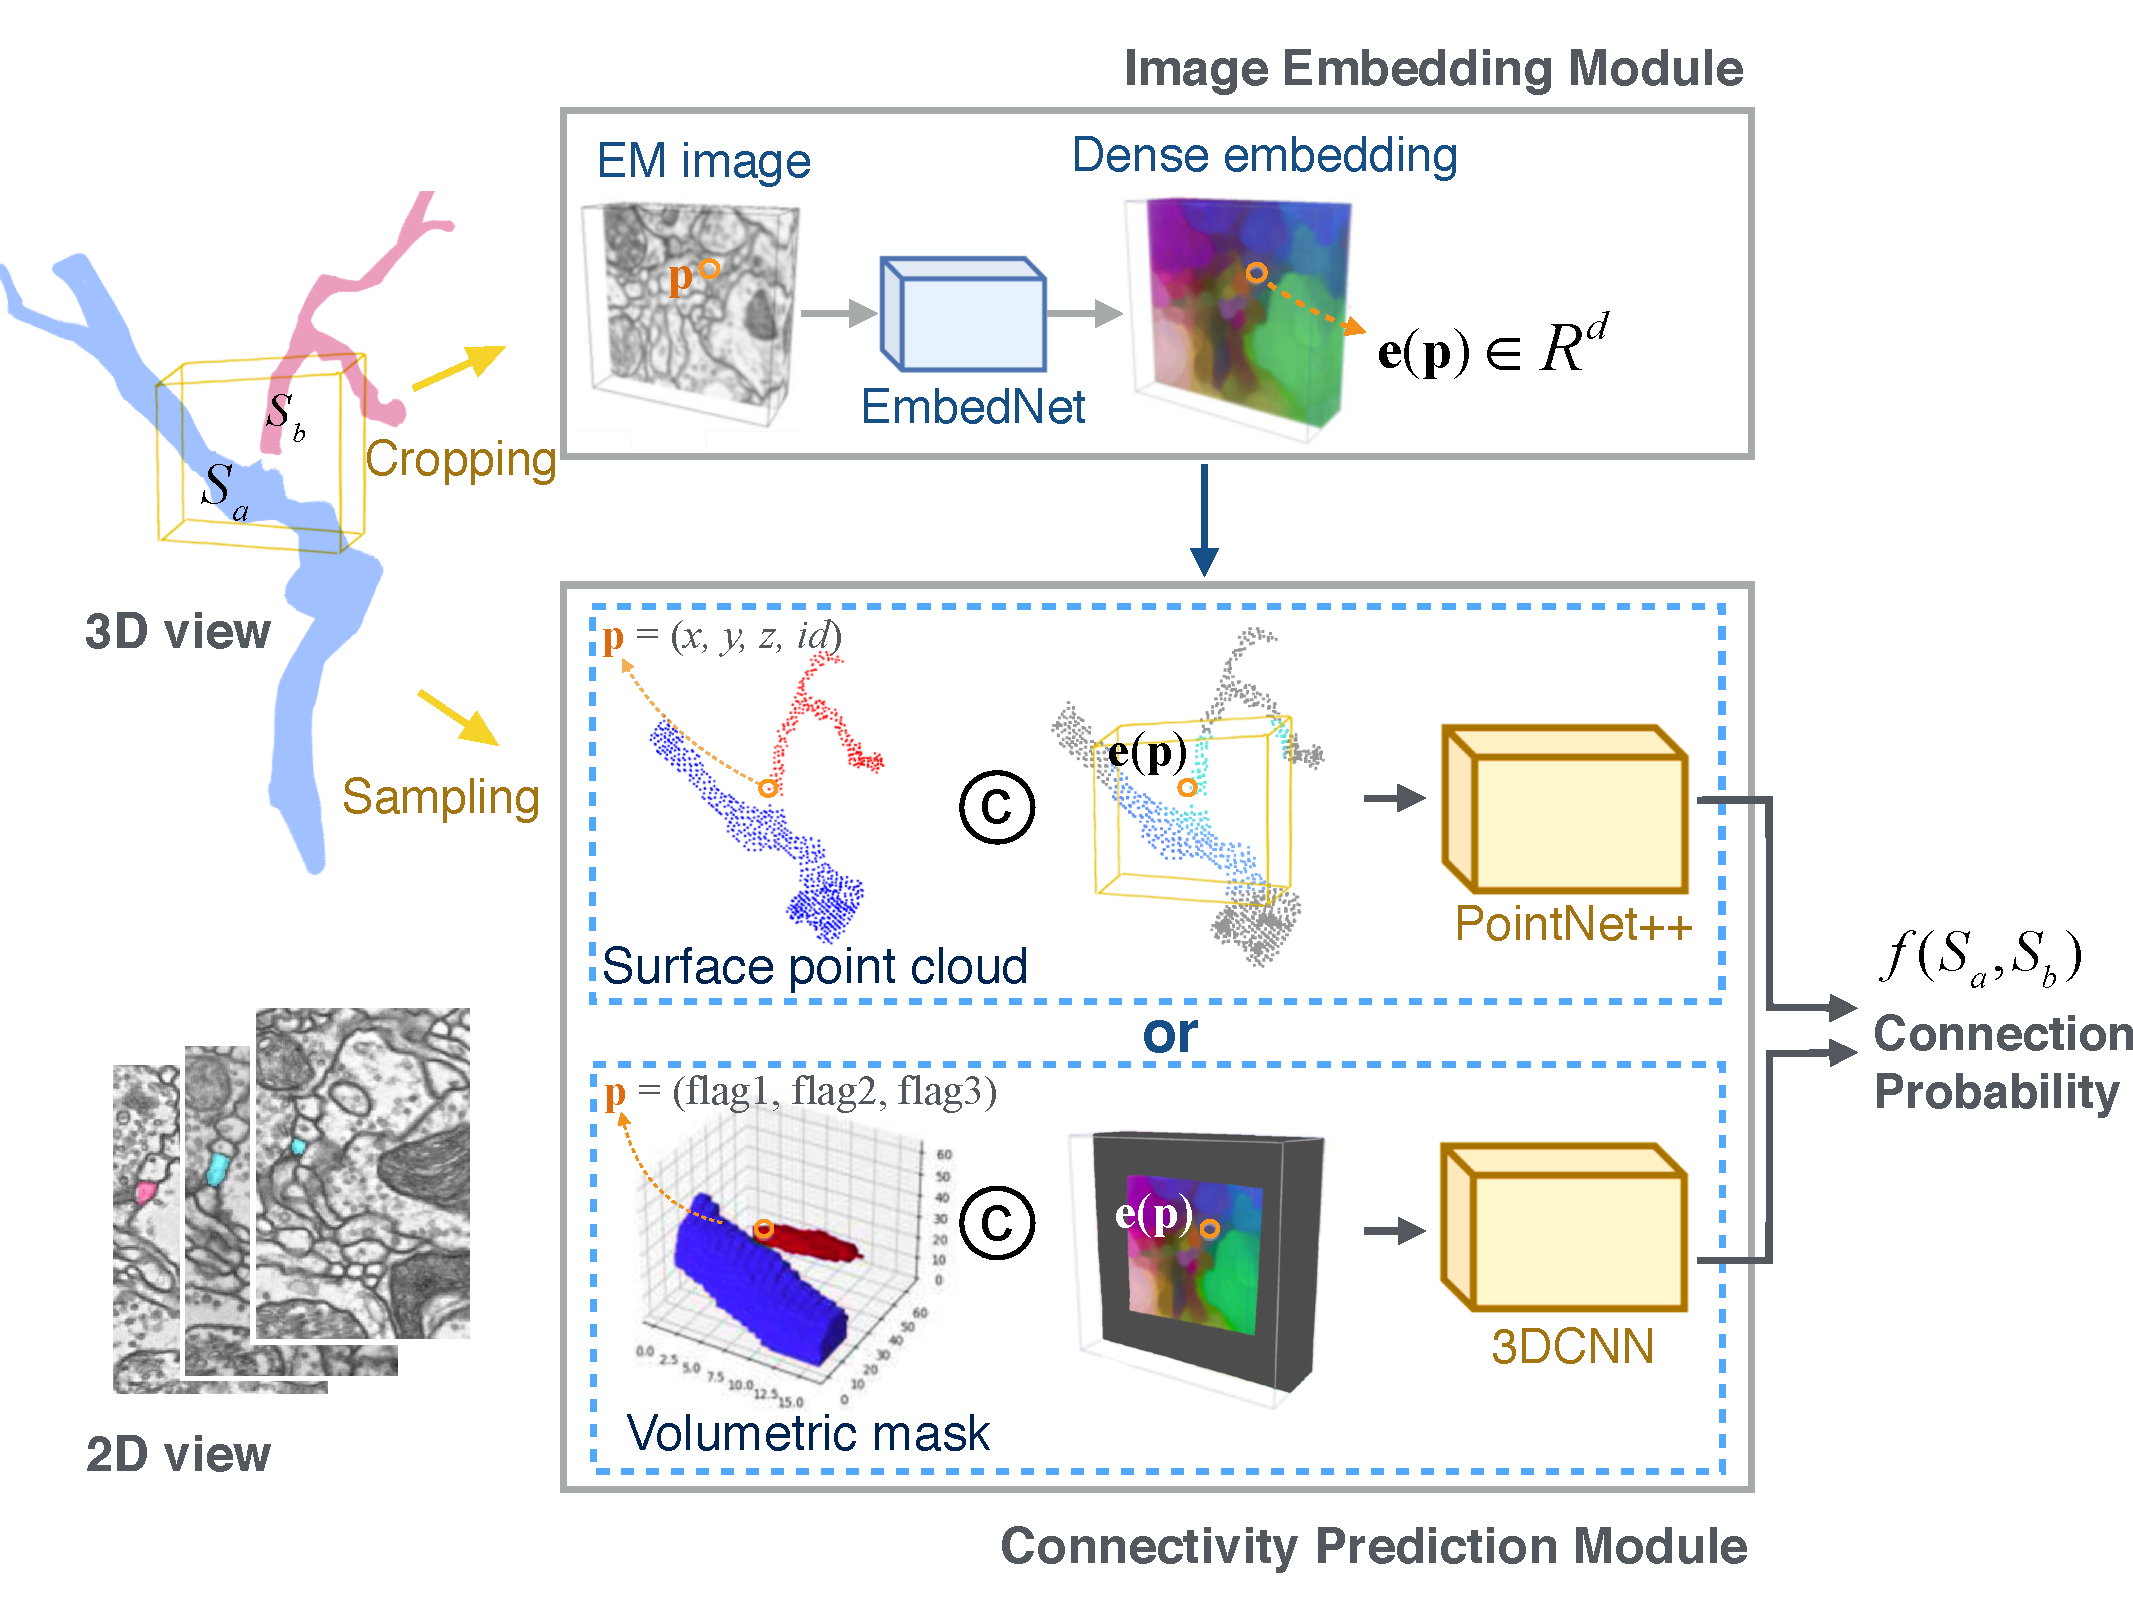
\includegraphics[width=0.48\textwidth]{figs/3Dmodel.pdf}
    \caption{Our connectivity prediction framework fuses local volumetric image features extracted by the EmbedNet with 3D morphology, optionally represented by point cloud or volumetric masks.}% 
    \label{fig:3Dmodel}
\end{figure}

Consequently, we collect the entire bridging edge set from $23,769$ proofread neurons.
The average count of bridging edges per neuron is 810. 
%
For each bridging edge $edge(\mathbf{v}_i, \mathbf{v}_j)$, assuming ${\mathbf{c}}_{i,j}$ is the midpoint of $\mathbf{v}_i$ and $\mathbf{v}_j$, we add random shift to the coordinate of ${\mathbf{c}}_{i,j}$ and obtain ${\hat{\mathbf{c}}}_{i,j}$ as the estimated truncated point. 
The segment pair $(S_a, S_b)$ is annotated as a positive connecting pair ($f(S_a, S_b)=1$).
Any segment $S_c$ that is located in the cube of size $H\times W\times D$ centered at ${\hat{\mathbf{c}}}_{i,j}$ and $S_c \neq S_b$ is labeled with $S_a$ as a negative pair ($f(S_a, S_c)=0$). 


 \subsubsection{Training and Test Block Partition.}
The positive segment pairs across the entire fly brain are partitioned into blocks based on their location in the brain, each spanning a volume size of $26\times 26\times 1\mu m^3$. We select $4,000$ blocks, each of which contains a minimum of $350$ positive segment pairs for training and testing. 
 $1,000$ blocks are selected randomly as the training and validation set for the image embedding network and pairwise connectivity prediction models. The rest $3,000$ blocks are used for testing of connectivity prediction.
 
 

\section{Commonsense for Zero-Shot NLVL}
\label{sec:proposedSection}

\subsection{Problem Formulation}
We denote an input video as $V$, and its grounding annotations as \(\left( Q,V_{\text{span}}\right) \), where $Q$ is the query representation and \(V_{\text{span}}\!=\!\left( t_{s},t_{e}\right)\) is the corresponding video moment span annotation, with \(t_{s}\) and \(t_{e}\) representing the start and end timestamps, respectively. Learning to localize a video moment conditioned on a query entails maximizing the expected log-likelihood of the model parameterized by \(\theta\). In its typical setting, this can be formulated as follows:
\begin{equation}
\label{eq:groundingOriginal}
    \theta ^{\ast }=\arg \max _{\theta } \mathbb{E}\left[ \log p_{\theta }\left(  V_{\text{span}} | V,Q\right) \right]. 
\end{equation}
In the zero-shot setting, the goal is to learn this task without parallel video-query annotations. Hence, the query and video moment annotations are derived from $V$, using a dynamic video moment proposal method followed by a pseudo-query generation mechanism. Formally,  \(V_{\text{span}}\,\!{=}\!\,f_{\text{span}}(V)\) and \(Q\,\!{=}\!\,f_{pq}(V_{\text{span}})\), where $f_{\text{span}}$ and $f_{\text{pq}}$ are video moment proposal and pseudo-query generation mechanisms, respectively. Given that $f_{\text{span}}$ and $f_{\text{pq}}$ are responsible for generating the annotations, the performance of the localization model heavily depends on the quality of these modules. Existing methods face challenges in aligning \(Q\) to \(V_{\text{span}}\) due to noise introduced by ungrounded pseudo-query generation mechanisms. 
To address this, we simplify \(f_{\text{pq}}\) while augmenting cross-modal understanding by leveraging external information in the form of a commonsense graph \(G_{C}(C, E)\) with \(n_c\) nodes, where \(C\!=\!\left\{c_{1}, c_{2}, \dots, c_{n_{C}}\right\}\) are the concept node vector representations and \(E\) is the set of weighted directed edges, respectively. Accordingly, learning can be formulated as
\begin{equation}
\label{eq:groundingOurs}
    \theta ^{\ast }=\arg \max _{\theta } \mathbb{E}\left[ \log p_{\theta }\left(  V_{\text{span}}| V,Q,G_{C}\right) \right].
\end{equation}

\noindent Figure \ref{fig:approach} shows both training and inference flows.
\subsection{Pseudo-supervised Setup}
\modelname first processes a raw video with a video moment proposal $f_{\text{span}}$ module that extracts important video segments capturing key events, and a pseudo-query generation $f_{\text{pq}}$ that generates text query annotations corresponding to the extracted video segments.

\paragraph{Dynamic Video Moment Proposal ($f_{\text{span}}$).}
We adopt the dynamic video moment proposal approach proposed by \citet{nam_zero-shot_2021}. Specifically, $f_{\text{span}}$ primarily comprises a k-means clustering mechanism that groups semantically similar and temporally proximal video frame features together to extract atomic moments. To obtain frame features, we consider the columns of a frame-wise similarity matrix derived from the CNN features of individual frames. We enforce temporal proximity by concatenating the frame index to the features. Composite video moments are then formed by combining neighboring atomic moments, and a subset of all possible combinations is sampled uniformly at random. The resulting set of video moments corresponds to $V_{\text{span}}$.

\paragraph{Pseudo-query Generation ($f_{\text{pq}}$).} The pseudo-query is constructed as a collection of objects present in the video. To generate the pseudo-query, we employ an off-the-shelf object detector, enabling the extraction of pertinent objects in \(V_{\text{span}}\). We adopt a top-$k$ strategy to sample the $k$ most probable object predictions associated with the query \query.

\paragraph{Video Encoder.}
We uniformly sample $T$ frames from $V$ and extract their CNN (\eg, I3D~\cite{qian_locate_2022}) features. These features are contextually encoded using a video encoder ${\phi}_{v}$ to yield frame features ${\phi}_{v}(V)\!=\!\left\{ v_{1},v_{2},\ldots,v_{T}\right\}$ where $v_{i}\in\mathbb{R}^{d}$, and $d$ is the common video/query encoding dimension. We implement ${\phi}_{v}$ as a GRU-based encoder.

\paragraph{Query Encoder.}
Our pseudo-query $Q$, composed of up to $k$ tokens, is encoded using a query encoder ${\phi}_{q}$ that generates query embeddings ${\phi}_{q}(Q)\!=\!\left\{ q_{1},q_{2},\ldots,q_{k}\right\}$, for the top-$k$ detected objects extracted from the pseudo-query generation. Here, $q_{i}\in \mathbb{R}^{d}$ and $d$ is the common video/query encoding dimension. We implement ${\phi}_{q}$ as a bi-directional GRU-based encoder preceded by a trainable embedding layer. 

\subsection{Commonsense Enhancement Module}
\label{sec:cem}
To enrich the encoded video and query features with information grounded in commonsensical knowledge, we introduce a Commonsense Enhancement Module (CEM), pictorially described in Figure~\ref{fig:cem}. This enhancement helps inject necessary information into video and query representations, which can not just help bridge the gap between the available visual and textual cues but also provide rich information to the downstream span localization module. 

\begin{figure}[t!]
    \centering
    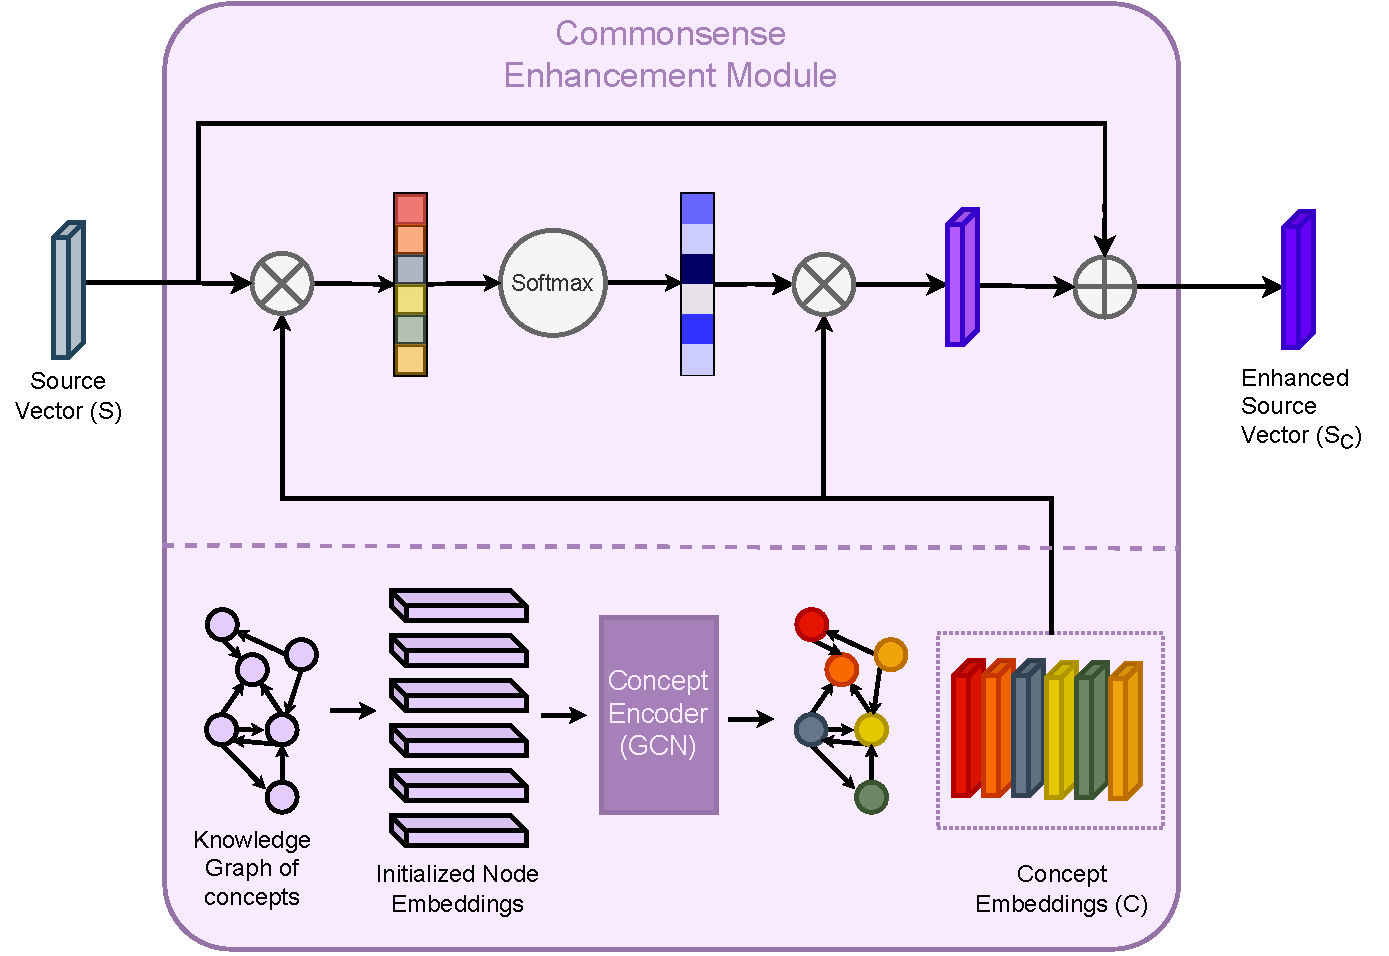
\includegraphics[width=0.8\linewidth]{figures/figure_files/Cem.pdf}
    \caption{\modelname Commonsense Enhancement Module (CEM). CEM comprises a concept encoder and an enhancement mechanism that uses the previously encoded concept vectors to update a given input vector (video/query vectors). The concept encoder employs a Graph Convolution Network for encoding the nodes (concepts) of \(G_C\). 
    }
  \label{fig:cem}
\end{figure}

CEM includes a set \(C\!=\!\left\{c_{1}, c_{2}, \dots, c_{n_{C}}\right\}\) of \(n_{C}\) concept vectors, where \(c_{i} \in \mathbb{R}^{d}\) and \(d\) is the concept feature dimension (same dimension as $\forall v_i \in V$ and $\forall q_i \in Q$). In general, given source feature vectors $S\!=\!\left\{ s_{1},s_{2},\ldots,s_{n}\right\}$ with individual feature vectors $s_{i \in [1,n]} \in \mathbb{R}^{d}$, the enhanced feature vectors $S_{C}$ are obtained using a commonsense enhancement mechanism $\phi_{C}$.
We implement this commonsense enhancement step $\phi_{C}$ as a cross-attention mechanism that enriches source input features, attending over $S$ guided by the commonsense concept vectors $C$, \ie, 
\begin{equation}
\label{eq:cenhance}
\scalemath{1}{
    }
    S_{C} = S + \phi_{C}(S) = S + \sigma \left( \frac{SW_{Q}(CW_{K})^{T}}{\sqrt{d}} \right) C W_{V},
\end{equation}
where $\sigma$ is a softmax activation, \(W_{Q}\), \(W_{K}\), \(W_{V}\) are trainable matrices and \(d\) is the common dimension of the vectors \(S\) and \(C\). In our setting, the source feature vectors $S$ are either video $V$ or pseudo-query $Q$ features. We build separate enhancement mechanisms for $V$ and $Q$, \ie, the projection matrices \(W_{Q}\), \(W_{K}\), \(W_{V}\) are not shared between $Q$ and $V$. We elaborate more on the rationale in the appendix.
The enriched video and pseudo-query features are denoted as \(V_{C}\!=\!\phi_{C_{\text{vid}}}(V)\) and \(Q_{C}\!=\!\phi_{C_{\text{pq}}}(Q)\), respectively.

\paragraph{Concept Encoder.}
The concept vectors \(C\) mentioned above are feature representations that internally form the nodes of the commonsense graph, \(G_C\). Accordingly, graph \(G_{C}\) is represented as a matrix, where \(G_{C(i,j)}\) represents the total number of directed relational edges between \(c_{i},c{j} \in C\) that start at \(c_i\) and end at \(c_j\). To encode the commonsense information, we employ Graph Convolutional Networks (GCN) \cite{hammond_wavelets_2011}. The concept encoder is composed of $L$ graph convolution layers, each of which performs a convolution step
\begin{equation}
\scalemath{1}{
    C^{\left(l+1\right)}=\sigma \left( AC^{\left(l\right) }W^{\left( l\right) }\right),
    }
\end{equation}
where $C^{\left(l\right)}$ are node (concept) features and $W^{\left( l\right)}$ trainable weight matrix of layer $l \in [1, L]$, $\sigma$ is a nonlinear activation function, and $A$ is the adjacency matrix obtained by normalizing graph $G_C$ with the degree matrix $D$. Since $G_C$ is a directed graph, normalization can be formulated as $A\!=\!D^{-1}G_{C}$.

\paragraph{Commonsense Information.}
We use ConceptNet \cite{speer_conceptnet_2017}, a popular knowledge graph that provides information spanning various types of relationships such as physical, spatial, behavioral, \etc To ensure that the ConceptNet information utilized is relevant to themes found in the video data, we consider the set of objects available in pseudo-queries and include the top-$k$ most frequently occurring objects to be the seed concept set \(C\). We extract the  ConceptNet subgraph that includes all edges incident between the concepts in \(C\). 
We filter the edge types based on a pre-determined relation set \(R\), which is compiled to involve relations that are relevant to the nature of the video localization task, \eg, spatial (\textit{AtLocation}, \etc) and temporal (\textit{HasSubevent}, \etc) relations are useful for video understanding, while \textit{RelatedTo} and \textit{Synonym} are fairly generic relations that add little information to the localization task. Table \ref{tab:relations} shows the relations included in \(G_C\).

\paragraph{Cross-Modal Interaction Module.} The commonsense enriched video and query features, \(V_{C}\) and \(Q_{C}\), are fused with a multi-modal cross-attention mechanism. We employ a two-step fusion process. First, Query-guided Video Attention (QVA) is applied to attend over video $V_C$, and Video-guided Query Attention (VQA) attends over query $Q_C$ guided by video $V_C$, resulting in updated features $V_C'$ and $Q_C'$, respectively. Both QVA and VQA utilize Attention Dynamic Filters~\cite{rodriguez_proposal-free_2020} that adaptively modify video features, dynamically adjusting them in response to the query, and vice versa. Next, the attended features are fused using a cross-attention mechanism over $V_C'$ guided by $Q_C'$, resulting in localized video features $V_{C_{\text{loc}}}$.

\paragraph{Temporal Regression Module.}
The final step involves a regression layer that approximates $\hat{V}_{\text{span}}$. We employ attention-guided temporal regression to estimate the span of the target video moment. To find important temporal segments relevant to the query, the fused features $V_{C_{\text{loc}}}$ are temporally attended based on the query features to obtain $V_{\text{ta}}$. Then, the span boundaries are localized using a regressor implemented as a Multi-Layer Perceptron (MLP).

\begin{align}
{o}_i = \sigma\left({W}_{1} V_{C_{\text{loc}_i}} + {b}_{{1}}\right) \\
V_{\text{ta}} = \sum_{i=1}^{T} o_i V_{C_{\text{loc}_{i}}} \\
[\hat{t}_s, \hat{t}_e] = {W}_2 {V}_{\text{ta}} + {b}_{2}.
\end{align}
Here, ${W}_{1}$ and ${b}_1$ are the weight matrix and bias vector of the temporal attention MLP, $\sigma$ represents the sigmoid activation function, $V_{C_{\text{loc}_i}}$ stands for the encoded localized video features, ${V}_{\text{ta}}$ represents the temporally attended video features, ${W}_2$ and ${b}_2$ denote the weight matrix and bias vector of the regression MLP, and $[\hat{t}_s, \hat{t}_e]$ correspond to the start and end timestamps of the predicted video span $\hat{V}_{\text{span}}$.

\begin{table}[t!]
\centering
\resizebox{\linewidth}{!}{
\begin{tabular}{ll}
\toprule
\textbf{Category} & \textbf{Relations}                                                                                         \\ \toprule
Spatial           & AtLocation, LocatedNear                                                                                    \\ \midrule
Temporal          & \begin{tabular}[c]{@{}l@{}}HasSubevent, HasFirstSubevent, HasLastSubevent, HasPrerequisite\end{tabular} \\ \midrule
Functional        & UsedFor                                                                                                    \\ \midrule
Causal            & Causes                                                                                                     \\ \midrule
Motivation        & MotivatedByGoal,  ObstructedBy                                                                             \\ \midrule
Other             & CreatedBy, MadeOf                                                                                          \\ \midrule
Physical          & \begin{tabular}[c]{@{}l@{}}HasA, HasProperty, Antonym, SimilarTo\end{tabular}                      
\\ \bottomrule
\end{tabular}
}

\caption{Relations in the Commonsense Enhancement Module (CEM) grouped by categories.}
\label{tab:relations}

\end{table}
\subsection{Training and Inference}
The training objective is 
$\mathcal{L}_{loc} = \mathcal{L}_{treg}+\lambda \mathcal{L}_{ta},$ where \(\lambda\) is a balancing hyperparameter, \(\mathcal{L}_{ta}\) is a temporal attention guided loss and \(\mathcal{L}_{treg}\) is the regression loss.  The temporal attention-guided loss is defined as
\begin{equation}
\label{tatt}
\mathcal{L}_{ta} = \frac{\sum^{T}_{i=1}g_{i}\log \left( a_{i}\right)}{\sum^{T}_{i=1}g_{i}},
\end{equation}
where \(a_{i}\) is the attention weight for video frame \(v_{i}\) and \(g_{i}\) is the attention mask for \(v_{i}\), that is assigned to \(1\) if \(v_{i}\) is inside the target video segment, and \(0\) otherwise. 
This objective encourages the model to produce higher attention weights for video segments that are relevant to the query. 
On the other hand, \(\mathcal{L}_{treg}\) dictates the video span boundary regression and is the sum of smooth $\ell_1$ distances between start and end timestamps of the ground truth and predicted spans, \ie,
\begin{equation}
\label{treg}
\mathcal{L}_{treg} = \text{smooth}{\ell_1}(t_{s}, \hat{t}_{s}) + \text{smooth}{\ell_1}(t_{e}, \hat{t}_{e}).
\end{equation}
Here, $t_{s}$ and ${t}_{e}$ represent the ground truth start and end timestamps and $\hat{t}_{s}$ and $\hat{t}_{e}$ the predicted start and end timestamps, respectively.
The integration of a smoothing mechanism enhances training stability and improves the model's ability to handle outliers. Finally, during inference, we employ an off-the-shelf part-of-speech tagger to extract nouns from the text input query and feed them as query input to the trained \modelname video localizer.


\section{Experiments}
\label{sec:experiment}

\begin{table}[t]
\centering
\small
\resizebox{0.99\linewidth}{!}{
\begin{tabular}{lcccc}
\multirow{2}{1.5cm}{\textbf{Methods}} & \multicolumn{2}{c}{\textbf{Far-OOD}} & \multicolumn{2}{c}{\textbf{Near-OOD}}\\
\cmidrule{2-5}
& \textbf{FPR95}  & \textbf{AUROC} & \textbf{FPR95}  & \textbf{AUROC}\\
& $\downarrow$ & $\uparrow$ & $\downarrow$ & $\uparrow$ \\
\toprule
\emph{Using model outputs}\\
MSP~\cite{hendrycks2016baseline} & 52.11 & 91.79 & 64.66 & 85.28 \\
ODIN~\cite{liang2018enhancing}  & 26.47 & 94.48 & 52.32 & 88.90\\
GODIN~\cite{hsu2020generalized}  & 17.42  & 95.84 & 60.69 & 82.37 \\
Energy score~\cite{liu2020energy}  & 28.40 & 94.22 & 50.64 & 88.66 \\
ReAct~\cite{sun2021react} & 33.12 & 94.32 & 53.51 & 88.96\\
GradNorm~\cite{huang2021importance} & 24.79 & 92.58 & 65.44 & 79.31\\
LogitNorm~\cite{wei2022mitigating}  & 19.61 & 95.51 & 55.08 & 88.03\\
DICE~\cite{sun2022dice}  & 20.83 & 95.24 & 58.60 & 87.11 \\
\midrule
\emph{Using feature representations}\\
Mahalanobis~\cite{lee2018simple} & 44.55 & 82.56 & 87.71 & 78.93 \\
KNN~\cite{sun2022knn}  & 18.50 & 96.36 & 58.34 & 87.90 \\
\midrule 
 \name (ours) & \textbf{14.99} & \textbf{97.15}  & \textbf{50.10} &  \textbf{89.80}\\
 & $\pm{0.87}$ & $\pm{0.27}$ & $\pm{1.09}$ & $\pm{0.65}$\\
\bottomrule
\end{tabular}}
\caption{\small Performance comparison on near-OOD and far-OOD detection task. Architecture used is DenseNet-101 and ID data is CIFAR-10. We report the mean and variance across 3 training runs.}
\label{tab:hard_ood}
\end{table}
\begin{table}[t]
\small
\centering
\resizebox{0.99\linewidth}{!}{
\begin{tabular}{lccc}
\textbf{Method} & \textbf{FPR95}  & \textbf{AUROC} & \textbf{ID Acc.}\\
& $\downarrow$ & $\uparrow$ & $\uparrow$ \\
\toprule
\emph{Methods using model outputs}\\
MSP~\cite{hendrycks2016baseline} & 77.59 & 76.47 &  75.14\\
ODIN~\cite{liang2018enhancing} & 56.39 & 86.02 & 75.14\\
GODIN~\cite{hsu2020generalized} & 44.08 &  89.05 & 74.37\\
Energy score~\cite{liu2020energy} & 57.07 &  84.83 &  75.14\\
ReAct~\cite{sun2021react} & 75.06 & 79.51 & 66.56\\
GradNorm~\cite{huang2021importance} & 63.05 & 79.80 & 75.14\\
LogitNorm~\cite{wei2022mitigating} & 61.10 & 84.72 & 75.42\\
DICE~\cite{sun2022dice} & 49.72 & 87.23 & 68.65 \\
\midrule 
\emph{Methods using feature representations}\\
Mahalanobis~\cite{lee2018simple} & 56.93 & 80.27 &  75.14\\
KNN~\cite{sun2022knn} & 47.21 & 85.27 & 75.14\\
\midrule 
 \name (ours) & \textbf{31.25} & \textbf{90.76} & \textbf{75.59}\\
& $\pm{1.25}$ & $\pm{0.36}$ & $\pm{0.08}$\\
\bottomrule
\end{tabular}}
\caption{\small Performance comparison on CIFAR-100 dataset. We use DenseNet-101 for all baselines. Best  results are in \textbf{bold}. We report the mean and variance across 3 different training runs.}
\label{tab:cifar-100}
\end{table}
In this section, we extensively evaluate the effectiveness of our proposed method. 
The goal of our experimental sections is to mainly answer the following questions: (1) Can \name alleviate the curse of dimensionality? (2) How does \name compare against the state-of-the-art OOD detection methods?  Due to space constraints, extensive experimental details are in Appendix C. Our code is open-sourced for the research community.


\subsection{Evaluation on Common Benchmarks}
\label{subsec:common_benchmark}

\noindent \textbf{Datasets.} In this section, we make use of commonly studied CIFAR-10 (10 classes) and CIFAR-100 (100 classes)~\cite{krizhevsky2009learning} datasets as ID. Both datasets consist of images of size $32 \times 32$. We use the standard split with $50,000$ images for training and $10,000$ images for testing. We evaluate the methods on common OOD datasets: \texttt{Textures}~\cite{cimpoi2014describing}, \texttt{SVHN}~\cite{svhn}, \texttt{LSUN-Crop}~\cite{yu2015lsun}, \texttt{LSUN-Resize}~\cite{yu2015lsun}, \texttt{iSUN}~\cite{xu2015turkergaze}, and \texttt{Places365}~\cite{zhou2017places}. Images in all these test datasets are of size $32 \times 32$. 


\paragraph{Evaluation metrics.} We compare the performance of various methods using the following metrics: 
(1) {FPR95} measures the false positive rate (FPR) of OOD samples when $95\%$ of ID samples are correctly classified;
(2) {AUROC} is the area under the Receiver Operating Characteristic curve; 
and (3) {ID Acc.} measures the ID classification accuracy.

\vspace{0.2cm}
\noindent \textbf{Comparison with competitive methods.} In Table~\ref{tab:cifar-100}, we provide a comprehensive comparison with competitive OOD detection baselines on  CIFAR-100. {We provide a detailed description of baseline approaches in Appendix C.3.} We observe that our proposed method \name significantly outperforms the latest rivals. For a fair comparison, we divide the baselines into two categories: methods using model outputs and methods using feature representations.
From Table~\ref{tab:cifar-100}, we highlight two salient observations: (1) Considering methods based on feature representations, \name outperforms KNN (non-parametric) and Mahalanobis (parametric) by \textbf{15.96\%} and \textbf{25.68\%} respectively in terms on FPR95. The results validate that learning feature subspace effectively alleviates the ``curse-of-dimensionality" problem that is troubling the existing KNN approach. (2) Further, \name also performs better than output-based methods such as ReAct~\cite{sun2021react}. Specifically, with CIFAR-100 as ID, \name provides a $\mathbf{43.81}\%$ improvement in FPR95 as compared to ReAct~\cite{sun2021react}. Notably, \name provides a \textbf{18.47\%} improvement compared to~\cite{sun2022dice}, a post-hoc sparsification method. While DICE can severely affect the ID test accuracy (68.65\%), \name exhibits stronger classification performance (75.59\%) by baking in the inductive bias of subspaces through training. An extensive discussion is provided in Section~\ref{sec:discussion}. 



\paragraph{Evaluation on near-OOD data.} In Table~\ref{tab:hard_ood}, we compare the performance in detecting near-OOD data, which refers to samples near the ID data. Near-OOD is particularly challenging to detect, and can often be misclassified as ID. We report the performance on CIFAR-10 (ID) vs. CIFAR-100 (OOD), which is the most commonly used dataset pair for this task. We observe that \name consistently outperforms existing algorithms for near-OOD detection tasks, further demonstrating its strengths. Compared to KNN, \name reduces the FPR95 by 8.24\%. For completeness, we also provide far-OOD evaluation results on CIFAR-10, where \name achieves an average FPR95 of 14.99\%. Full result on each test dataset for CIFAR-10 is available in Appendix D.4.



\begin{table}[t]
\small
\centering
\resizebox{0.95\linewidth}{!}{
\begin{tabular}{lccc}
\textbf{Method} & \textbf{Dataset (ID)} & \textbf{FPR95}  & \textbf{AUROC} \\
& & $\downarrow$ & $\uparrow$  \\
\toprule
Mahalanobis~\cite{lee2018simple} & CIFAR-10 & 44.55 & 82.56  \\

\name (w. Mahalanobis) & CIFAR-10 &  \textbf{34.68} &  \textbf{87.87} \\
\midrule
Mahalanobis~\cite{lee2018simple} & CIFAR-100 & 56.93 & 80.27  \\

\name (w. Mahalanobis) & CIFAR-100 &  \textbf{55.05} &  \textbf{80.77} \\
\bottomrule
\end{tabular}}
\caption{\small \name is also compatible with parametric approaches such as Mahalanobis distance~\cite{lee2018simple}. The model is DenseNet. All values are averaged over six OOD test datasets.}
\label{tab:compatibility}
\end{table}


\paragraph{Compatibility with other distance-based approaches.} 

Beyond KNN~\cite{sun2022knn}, the Mahalanobis distances~\cite{lee2018simple} is also one of the most popular distance-based approaches to detect OOD. 
However, all prior solutions measure the distance with a full feature space which can also suffer from the curse of dimensionality. 
In this section, we show that subspace learning can also benefit parametric approaches like Mahalanobis distance~\cite{lee2018simple}. In Table~\ref{tab:compatibility}, we compare the OOD detection performance of using Mahalanobis distance on the vanilla model and the model trained with \name. 
We see that coupling subspace learning (in training) with Mahalanobis distance (in testing) reduces FPR95 by {9.87\%} and {1.88\%} on CIFAR-10 and CIFAR-100 datasets respectively.

\begin{table}[t]
\small
\centering
\resizebox{0.55\linewidth}{!}{
\begin{tabular}{lcc}
\toprule
\multirow{2}{2cm}{\textbf{Training Method}} &  CIFAR-10 & CIFAR-100 \\ 
& \multicolumn{2}{c}{(Train time in hours)} \\
\midrule
Standard & $2.10$ & $2.25$\\ 
 \name & $1.75$ & $1.89$ \\
\bottomrule
\end{tabular}}
\caption{\small \textbf{Computational cost for training}. trained using ResNet-101. 
Model used is DenseNet-101. For the comparison, we used the software configuration as reported in Appendix C.2.}
\label{tab:train_time}
\end{table}
% 
\paragraph{Computational complexity.}  In Table~\ref{tab:train_time}, we compare the training time of \name with the standard training method using cross-entropy loss. We observe that training using \name incurs no additional computation overhead but rather is slightly more efficient compared to standard training procedures. This is because we perform gradient descent only on a subset of weights corresponding to the selected feature subspace. Thus, our method overall leads to faster updates and convergence. {In Appendix D.1, we further show that
\name remains competitive and outperforms the KNN counterpart on other common architecture.}

\section{Related Work}

There are two major streams of literature that intersect with our problem: 1) shelf space allocation and 2) deep reinforcement learning for spatial allocation.

\subsection{Shelf Space Allocation} 
The shelf space allocation allocation problem has been studied in the operations research literature for many decades. Some classical work approaches the problem by proposing a dynamic programming algorithm to allocate limited shelf space among a finite set of products. In this case, the objective function is composed of revenue, costs and a set of constraints \cite{zufryden}. Later work proposed a simulated annealing optimization approach that accounts for two primary decisions variables: product assortment and allocated space for each product \cite{borin}. This optimization technique accounts for many different environment variables such as item profitability, brand elasticities, and supply chain features. More recently, frequent pattern mining algorithms have been proposed to allocate product shelf space. For instance Brijs et al. \cite{brijs} propose the PROFSET algorithm, which an association rule algorithm that mines customer basket sets to identify profitable product pairings. This algorithm is a extension of frequent item set algorithms that also accounts for product value. Extensions of this idea have also been proposed. Aloysius and Binu propose a PrefixSpan algorithm for shelf allocation  that first identifies complementary categories from historical purchase data before identifying product mix strategies within categories \cite{aloysius}.

These existing studies differ from our work in the following ways. First, they all focus on micro-regions (shelves) within the retail environment. The spatial effects these models capture are markedly different from the macro-level ones tackled in the current work. Second, these studies focus on the number of each product on a shelf. They try to maximize profitability given the fixed shelf volume. This optimization problem is fundamentally different from allocating products across the entire store. For these reasons, none of these methods can be directly applied to our problem.

\subsection{Deep Reinforcement Learning for Spatial Resource Allocation} Recent breakthroughs in reinforcement learning \cite{mnih} \cite{silver-16} \cite{silver-17} have spurred interest in RL as an optimization approach in complex and dynamic environments. In particular, recent studies have proposed RL algorithms as a mechanism for  spatiotemporal resource allocation.

\textbf{Order dispatching.} Significant attention has been paid to the order dispatching problem in ride sharing systems. Briefly, order dispatching refers to the problem of efficiently matching riders and drivers in an urban environment. The RL agent must learn the complex spatial dynamics to learn a policy to solve the dispatching problem. For example, Lin et al. \cite{lin-msu} tackle the dispatch problem by proposing a contextual multi-agent reinforcement learning framework that coordinates strategies among a large number of agents to improve driver allocation in physical space. Additionally, Li et al. \cite{li} also approach the order dispatching problem with multi-agent reinforcement learning (MARL). Their method relies on the mean field approximation to capture the dynamic, spatially distributed fluctuations in supply and demand. They empirically show that MARL can reduce supply-demand gaps in peak hours.

\textbf{Traffic signal control} Increasing traffic congestion is a key concern in many urban areas. Recent efforts to optimize traffic control systems via reinforcement learning has shown encouraging results. These systems seek to adjust traffic lights to real-time fluctuations in traffic volume and road demand. Wei et al \cite{intellilight} propose IntelliLight, which is a phase-gated deep neural network that approximates state-action values. More recently \cite{colight} proposes a graph attentional network to facilitate cooperation between many traffic signals.

\textbf{Spatial demand for electronic tolls} Chen et al. \cite{chen} propose a dynamic electronic toll collection system that adjusts to traffic patterns and spatial demand for roads in real time. Their proposed algorithm, PG-$\beta$, is an extension of policy gradient methods and decreases traffic volume and travel time.


While these reinforcement learning methods deal with the large-scale optimization of spatial resource, they cannot be directly applied to the product allocation problem because the all rely on domain-specific simulators. We propose our model in an effort to extend these state-of-the-art optimization techniques to our problem.

\section{Conclusion}
We curated \PyEnvs, a collection of permissively licensed Python packages along with isolated development environments.
Upon that, we built a function call argument completion dataset \CallArgs containing analyzer-induced information for each function call.
We experimented feeding auxiliary information as additional input context to various pretrained code language models for call argument completion during training and inference.
Results show that access to the function implementation and function usages universally improves the model performances.
We further provide insights on the effect of different types of models and different types of additional information on this task.
In the future, we can use \PyEnvs to construct new datasets for other code-related tasks to further study the benefits from cross-file and cross-project information.

Minus voluptatem tenetur at inventore odio iusto explicabo autem, iure repellendus saepe, officiis nihil aliquam debitis dolor minima suscipit et aperiam, dolor quia odio fugiat molestiae ea laudantium ipsam expedita aperiam.Sequi libero accusamus sapiente, quas ut dolores debitis perspiciatis non voluptatibus, quasi debitis eos adipisci nemo sit praesentium?Dolorem laudantium obcaecati numquam saepe perspiciatis voluptatem veritatis, quo molestiae fuga corrupti officia quidem eaque assumenda?Porro odit corporis doloribus aut recusandae delectus quaerat eligendi, amet officia ab fugiat eaque sit totam pariatur minus dignissimos.Corporis vel ab, nesciunt accusantium quibusdam ratione consequatur asperiores, earum alias aliquid repellat iusto quia nulla.Nesciunt voluptatibus perspiciatis, quod nulla amet ipsum neque vitae necessitatibus perferendis, nam quos molestias voluptates dignissimos ex doloremque.Nulla impedit optio exercitationem, repudiandae architecto molestias et sunt, similique fugit quam iure iste?Impedit fugit inventore laudantium laborum tempora possimus perspiciatis eligendi incidunt, temporibus similique laudantium consectetur soluta dignissimos necessitatibus modi distinctio, nesciunt magnam in eius?Praesentium molestias quo in soluta, tempora fugit accusantium eius aliquam, eos vero laboriosam adipisci ducimus recusandae sit in aperiam amet voluptatum, iusto doloremque dolores nihil quod reprehenderit corporis dolorum illo vel.\clearpage
\bibliography{main}



% Appendix is omitted for the camera-ready submission.


\end{document}